\documentclass[serif]{beamer}
%\usetheme{Berlin}

\usepackage[T1]{fontenc}
\usepackage{amsmath}
\usepackage{amssymb}
\usepackage{mathrsfs}
\usepackage{braket}
\usepackage{mathtools}
\usepackage{graphicx}
\usepackage{verbatim}
\usepackage{tikz}
\usetikzlibrary{decorations.pathreplacing}

\title{Conservation of Momentum}
\author{PH 211 Spring 2024}
\date{30 May 2024}

\newcommand{\Net}{\text{net}}
\newcommand{\Netext}{\text{net,ext}}
\newcommand{\Tot}{\text{total}}

\beamertemplatenavigationsymbolsempty

\newcommand{\MasterGuideSwitch}{1}
\newcommand{\Guides}[1][1]{
\begin{scope}
	\path (-5.3,4) -- (5.3,4) -- (5.3,-4) -- (-5.3,-4) -- cycle;
	\if0#1
	\else
	\if\MasterGuideSwitch0
	\else
	\draw[gray] (-5.3,4) -- (5.3,4) -- (5.3,-4) -- (-5.3,-4) -- cycle;
	\draw[gray] (-5.3,4) grid (5.3,-4);
	\draw[cyan] (-5.3,0) -- (5.3,0);
	\draw[cyan] (0,-4)--(0,4);
	\fi
	\fi
\end{scope}
}
\newcommand{\Bullet}[3][1]{
\begin{scope}[shift={(#2)}]
	\if0#1
	\node[anchor=west] at (0,0) {#3};
	\else
	\if1#1
	\filldraw[color=blue, fill=blue] (0,0) circle (2pt);
	\node[anchor=west] at (0,0) {#3};
	\else
	\if2#1
	\draw[blue, thick] (0.3,0) circle (2pt);
	\node[anchor=west] at (0.3,0) {#3};
	\else
	\draw[blue, ultra thick, shift={(0.6,0)}] (-2pt,0) -- (2pt,0);
	\node[anchor=west] at (0.6,0) {#3};
	\fi
	\fi
	\fi
\end{scope}
}

\begin{document}

%\frame{\titlepage}

\begin{frame}{Conservation of Momentum}
	\begin{figure}[h]
		\centering
		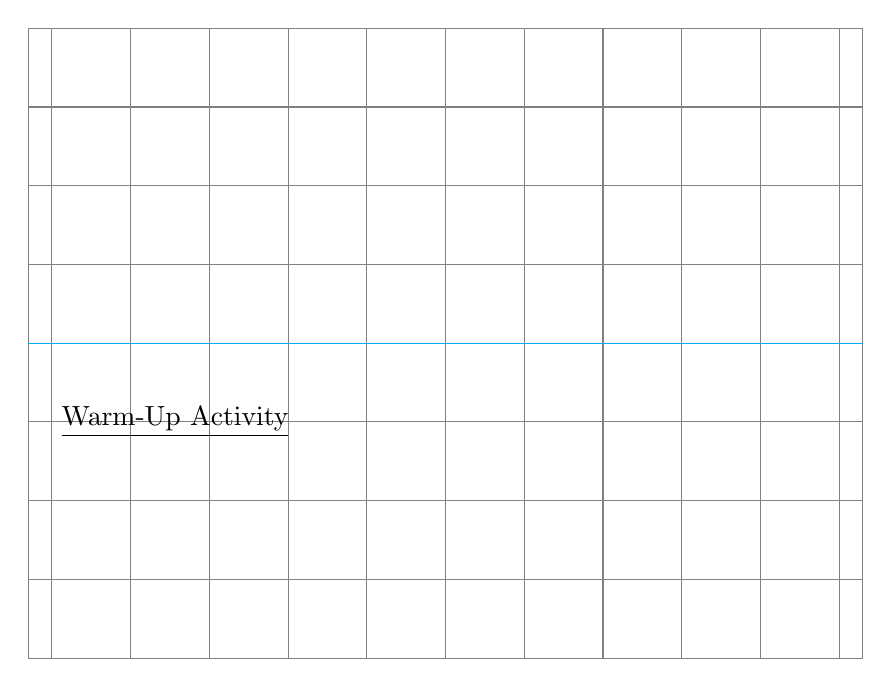
\begin{tikzpicture}
			\Guides%[0]
			\Bullet[0]{-5,-1}{\underline{Warm-Up Activity}}
		\end{tikzpicture}
	\end{figure}
\end{frame}

\begin{frame}{A Deeper Model for Interactions}
	\begin{figure}[h]
		\centering
		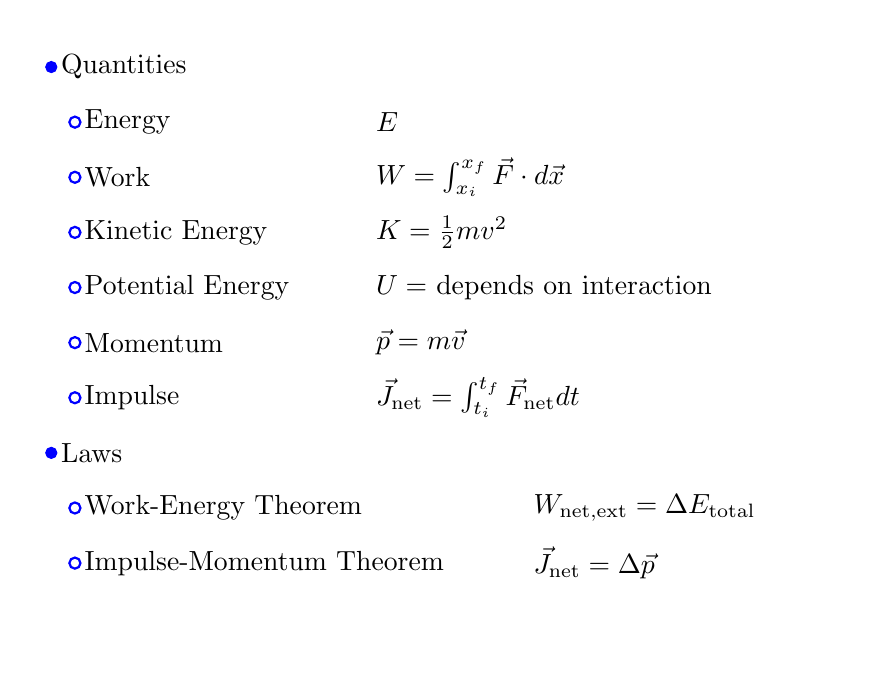
\begin{tikzpicture}
			\Guides[0]
			\Bullet{-5,3.5}{Quantities}
			\Bullet[2]{-5,2.8}{Energy}
			\Bullet[0]{-1,2.8}{$E$}
			\Bullet[2]{-5,2.1}{Work}
			\Bullet[0]{-1,2.1}{$W=\int_{x_{i}}^{x_{f}}\vec{F}\cdot d\vec{x}$}
			\Bullet[2]{-5,1.4}{Kinetic Energy}
			\Bullet[0]{-1,1.4}{$K=\frac{1}{2}mv^{2}$}
			\Bullet[2]{-5,0.7}{Potential Energy}
			\Bullet[0]{-1,0.7}{$U=$ depends on interaction}
			\Bullet[2]{-5,0}{Momentum}
			\Bullet[0]{-1,0}{$\vec{p}=m\vec{v}$}
			\Bullet[2]{-5,-0.7}{Impulse}
			\Bullet[0]{-1,-0.7}{$\vec{J}_{\Net}=\int_{t_{i}}^{t_{f}}\vec{F}_{\Net}dt$}
			\Bullet{-5,-1.4}{Laws}
			\Bullet[2]{-5,-2.1}{Work-Energy Theorem}
			\Bullet[0]{1,-2.1}{$W_{\Netext} = \Delta E_{\Tot}$}
			\Bullet[2]{-5,-2.8}{Impulse-Momentum Theorem}
			\Bullet[0]{1,-2.8}{$\vec{J}_{\Net}=\Delta\vec{p}$}
		\end{tikzpicture}
	\end{figure}
\end{frame}

\begin{frame}{Energy and Collisions}
	\begin{figure}[h]
		\centering
		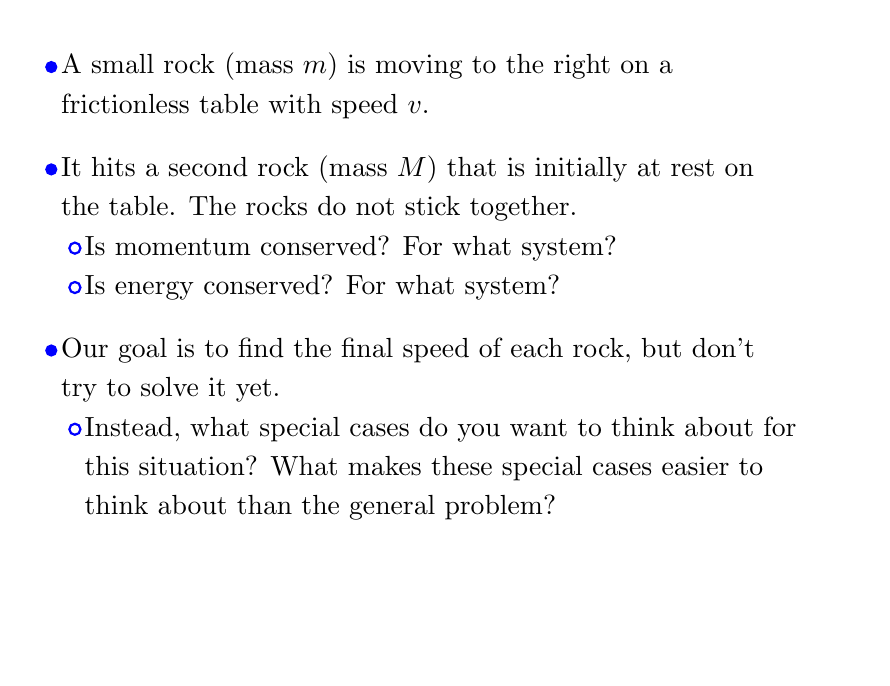
\begin{tikzpicture}
			\Guides[0]
			\Bullet{-5,3.5}{A small rock (mass $m$) is moving to the right on a}
			\Bullet[0]{-5,3}{frictionless table with speed $v$.}
			\begin{scope}[shift={(0,-0.3)}]
			\Bullet{-5,2.5}{It hits a second rock (mass $M$) that is initially at rest on}
			\Bullet[0]{-5,2}{the table. The rocks do not stick together.}
			\Bullet[2]{-5,1.5}{Is momentum conserved? For what system?}
			\Bullet[2]{-5,1}{Is energy conserved? For what system?}
			\end{scope}
			\begin{scope}[shift={(0,-0.6)}]
			\Bullet{-5,0.5}{Our goal is to find the final speed of each rock, but don't}
			\Bullet[0]{-5,0}{try to solve it yet.}
			\Bullet[2]{-5,-0.5}{Instead, what special cases do you want to think about for}
			\Bullet[0]{-4.7,-1}{this situation? What makes these special cases easier to}
			\Bullet[0]{-4.7,-1.5}{think about than the general problem?}
			\end{scope}
		\end{tikzpicture}
	\end{figure}
\end{frame}

\begin{frame}{Energy and Collisions}
	\begin{figure}[h]
		\centering
		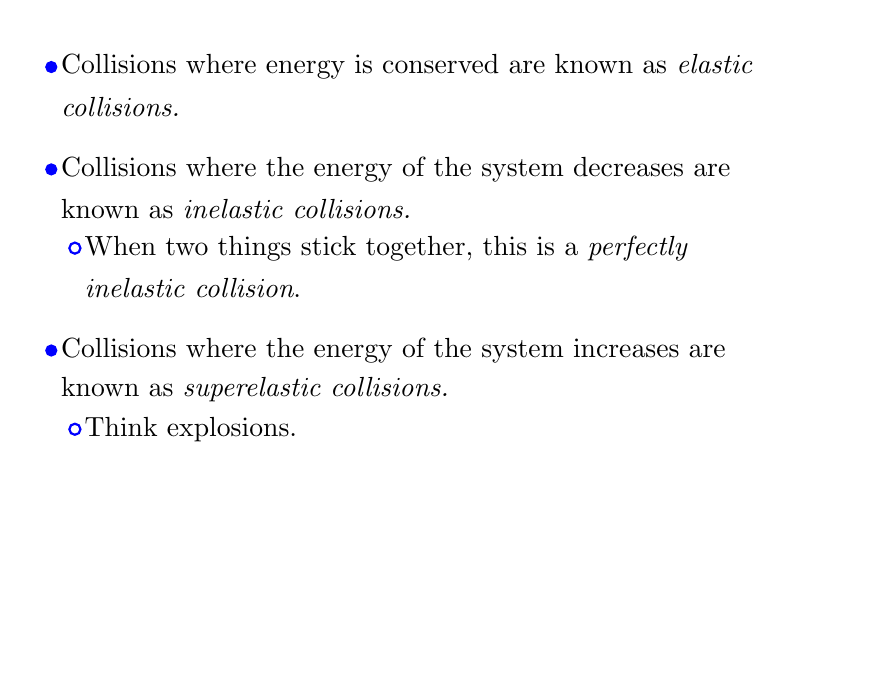
\begin{tikzpicture}
			\Guides[0]
			\Bullet{-5,3.5}{Collisions where energy is conserved are known as \textit{elastic}}
			\Bullet[0]{-5,3}{\textit{collisions.}}
			\Bullet{-5,2.2}{Collisions where the energy of the system decreases are}
			\Bullet[0]{-5,1.7}{known as \textit{inelastic collisions.}}
			\Bullet[2]{-5,1.2}{When two things stick together, this is a \textit{perfectly}}
			\Bullet[0]{-4.7,0.7}{\textit{inelastic collision}.}
			\Bullet{-5,-0.1}{Collisions where the energy of the system increases are}
			\Bullet[0]{-5,-0.6}{known as \textit{superelastic collisions.}}
			\Bullet[2]{-5,-1.1}{Think explosions.}
		\end{tikzpicture}
	\end{figure}
\end{frame}

\begin{frame}{Superelastic Collisions}
	\begin{figure}[h]
		\centering
		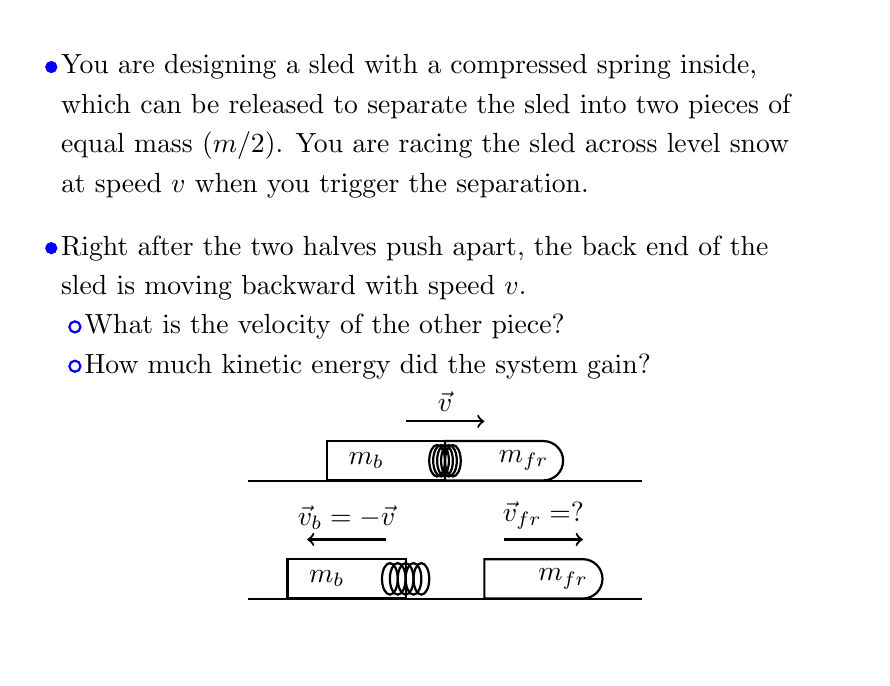
\begin{tikzpicture}
			\Guides[0]
			\Bullet{-5,3.5}{You are designing a sled with a compressed spring inside,}
			\Bullet[0]{-5,3}{which can be released to separate the sled into two pieces of}
			\Bullet[0]{-5,2.5}{equal mass ($m/2$). You are racing the sled across level snow}
			\Bullet[0]{-5,2}{at speed $v$ when you trigger the separation.}
			\begin{scope}[shift={(0,-1.3)}]
				\Bullet{-5,2.5}{Right after the two halves push apart, the back end of the}
				\Bullet[0]{-5,2}{sled is moving backward with speed $v$.}
				\Bullet[2]{-5,1.5}{What is the velocity of the other piece?}
				\Bullet[2]{-5,1}{How much kinetic energy did the system gain?}
			\end{scope}
			\begin{scope}[rotate=0,shift={(0,-1.5)}]
				\draw[thick,->] (-0.5,0.5) -- (0.5,0.5);
				\node[anchor=south] at (0,0.5) {$\vec{v}$};
				\begin{scope}
					\draw[thick] (-1.5,0.25) rectangle (0,-0.25);
					\node at (-1,0) {$m_{b}$};
				\end{scope}
				\begin{scope}
					\draw[thick] (0,0.25) -- (1.25,0.25) arc (90:-90:0.25) -- (0,-0.25) -- cycle;
					\node at (1,0) {$m_{fr}$};
				\end{scope}
				\begin{scope}[yscale=2]
					\newcommand{\Comp}{0.05}
					\draw[thick] ({-\Comp*2},0) circle (0.1);
					\draw[thick] (-\Comp,0) circle (0.1);
					\draw[thick] (0,0) circle (0.1);
					\draw[thick] (\Comp,0) circle (0.1);
					\draw[thick] ({\Comp*2},0) circle (0.1);
				\end{scope}
				\draw[thick] (-2.5,-0.26) -- (2.5,-0.26);
			\end{scope}
			\begin{scope}[rotate=0,shift={(0,-3)}]
				\begin{scope}[shift={(-0.5,0)}]
					\draw[thick,->] (-0.25,0.5) -- (-1.25,0.5);
					\node[anchor=south] at (-0.75,0.5) {$\vec{v}_{b}=-\vec{v}$};
					\draw[thick] (-1.5,0.25) rectangle (0,-0.25);
					\node at (-1,0) {$m_{b}$};
				\end{scope}
				\begin{scope}[shift={(0.5,0)}]
					\draw[thick,->] (0.25,0.5) -- (1.25,0.5);
					\node[anchor=south] at (0.75,0.5) {$\vec{v}_{fr}=$?};
					\draw[thick] (0,0.25) -- (1.25,0.25) arc (90:-90:0.25) -- (0,-0.25) -- cycle;
					\node at (1,0) {$m_{fr}$};
				\end{scope}
				\begin{scope}[yscale=2,shift={(-0.5,0)}]
					\newcommand{\Comp}{0.1}
					\draw[thick] ({-\Comp*2},0) circle (0.1);
					\draw[thick] (-\Comp,0) circle (0.1);
					\draw[thick] (0,0) circle (0.1);
					\draw[thick] (\Comp,0) circle (0.1);
					\draw[thick] ({\Comp*2},0) circle (0.1);
				\end{scope}
				\draw[thick] (-2.5,-0.26) -- (2.5,-0.26);
			\end{scope}
		\end{tikzpicture}
	\end{figure}
\end{frame}

\begin{frame}{Superelastic Collisions}
	\begin{figure}[h]
		\centering
		\begin{tikzpicture}
			\Guides[0]
			\Bullet{-5,3.5}{What if the sled is going up a hill?}
			\begin{scope}[shift={(-3,2)},rotate=30]
				\draw[thick,->] (-0.5,0.5) -- (0.5,0.5);
				\node[anchor=south] at (0,0.5) {$\vec{v}$};
				\begin{scope}
					\draw[thick] (-1.5,0.25) rectangle (0,-0.25);
					\node at (-1,0) {$m_{b}$};
				\end{scope}
				\begin{scope}
					\draw[thick] (0,0.25) -- (1.25,0.25) arc (90:-90:0.25) -- (0,-0.25) -- cycle;
					\node at (1,0) {\small$m_{fr}$};
				\end{scope}
				\begin{scope}[yscale=2]
					\newcommand{\Comp}{0.05}
					\draw[thick] ({-\Comp*2},0) circle (0.1);
					\draw[thick] (-\Comp,0) circle (0.1);
					\draw[thick] (0,0) circle (0.1);
					\draw[thick] (\Comp,0) circle (0.1);
					\draw[thick] ({\Comp*2},0) circle (0.1);
				\end{scope}
				\draw[thick] (-2.5,-0.26) -- (2.5,-0.26);
			\end{scope}
			\begin{scope}[shift={(3,2)},rotate=30]
				\begin{scope}[shift={(-0.5,0)}]
					\draw[thick,->] (-0.25,0.5) -- (-1.25,0.5);
					\node[anchor=south east] at (-0.75,0.5) {$\vec{v}_{b}=-\vec{v}$};
					\draw[thick] (-1.5,0.25) rectangle (0,-0.25);
					\node at (-1,0) {$m_{b}$};
				\end{scope}
				\begin{scope}[shift={(0.5,0)}]
					\draw[thick,->] (0.25,0.5) -- (1.25,0.5);
					\node[anchor=south east] at (0.75,0.5) {$\vec{v}_{fr}=$ ?};
					\draw[thick] (0,0.25) -- (1.25,0.25) arc (90:-90:0.25) -- (0,-0.25) -- cycle;
					\node at (1,0) {\small$m_{fr}$};
				\end{scope}
				\begin{scope}[yscale=2,shift={(-0.5,0)}]
					\newcommand{\Comp}{0.1}
					\draw[thick] ({-\Comp*2},0) circle (0.1);
					\draw[thick] (-\Comp,0) circle (0.1);
					\draw[thick] (0,0) circle (0.1);
					\draw[thick] (\Comp,0) circle (0.1);
					\draw[thick] ({\Comp*2},0) circle (0.1);
				\end{scope}
				\draw[thick] (-2.5,-0.26) -- (2.5,-0.26);
			\end{scope}
			\begin{onlyenv}<2->
			\Bullet{-5,0}{There is a net force, so impulse is not zero!}
			\Bullet[2]{-5,-0.4}{We need to know how long the}
			\Bullet[0]{-4.7,-0.8}{spring takes to decompress.}
			\end{onlyenv}
			\begin{onlyenv}<3>
			\Bullet{-5,3.5}{What if the sled is going up a hill?}
			\begin{scope}[shift={(-3,-2.5)},rotate=90]
				\draw[thick,->] (-0.5,0.5) -- (0.5,0.5);
				\node[anchor=east] at (0,0.5) {$\vec{v}$};
				\begin{scope}
					\draw[thick] (-1.5,0.25) rectangle (0,-0.25);
					\node at (-1,0) {$m_{b}$};
				\end{scope}
				\begin{scope}
					\draw[thick] (0,0.25) -- (1.25,0.25) arc (90:-90:0.25) -- (0,-0.25) -- cycle;
					\node at (1,0) {\tiny$m_{fr}$};
				\end{scope}
				\begin{scope}[yscale=2]
					\newcommand{\Comp}{0.05}
					\draw[thick] ({-\Comp*2},0) circle (0.1);
					\draw[thick] (-\Comp,0) circle (0.1);
					\draw[thick] (0,0) circle (0.1);
					\draw[thick] (\Comp,0) circle (0.1);
					\draw[thick] ({\Comp*2},0) circle (0.1);
				\end{scope}
			\end{scope}
			\begin{scope}[shift={(3,-2)},rotate=90]
				\begin{scope}[shift={(-0.5,0)}]
					\draw[thick,->] (-0.25,0.5) -- (-1.25,0.5);
					\node[anchor=east] at (-0.75,0.5) {$\vec{v}_{b}=-\vec{v}$};
					\draw[thick] (-1.5,0.25) rectangle (0,-0.25);
					\node at (-1,0) {$m_{b}$};
				\end{scope}
				\begin{scope}[shift={(0.5,0)}]
					\draw[thick,->] (0.25,0.5) -- (1.25,0.5);
					\node[anchor=east] at (0.75,0.5) {$\vec{v}_{fr}=$ ?};
					\draw[thick] (0,0.25) -- (1.25,0.25) arc (90:-90:0.25) -- (0,-0.25) -- cycle;
					\node at (1,0) {\tiny$m_{fr}$};
				\end{scope}
				\begin{scope}[yscale=2,shift={(-0.5,0)}]
					\newcommand{\Comp}{0.1}
					\draw[thick] ({-\Comp*2},0) circle (0.1);
					\draw[thick] (-\Comp,0) circle (0.1);
					\draw[thick] (0,0) circle (0.1);
					\draw[thick] (\Comp,0) circle (0.1);
					\draw[thick] ({\Comp*2},0) circle (0.1);
				\end{scope}
			\end{scope}
			\end{onlyenv}
		\end{tikzpicture}
	\end{figure}
\end{frame}

\begin{frame}{Main Ideas}
	\begin{figure}[h]
		\centering
		\begin{tikzpicture}
			\Guides[0]
			\Bullet{-5,2.5}{When the impulse is zero (because the net force is zero),}
			\Bullet[0]{-5,2}{the momentum of the system is constant---it is \textit{conserved}.}
		\end{tikzpicture}
	\end{figure}
\end{frame}

\end{document}
